\documentclass[11pt]{article}
	
%%%%%%%%%%%%%%%%%%%%%%%%%%%%%%%%%%%%%%%%%%%%%%%%%%%%%%%%%%%%%%%%%%%%%%
%\pdfminorversion=4
% NOTE: To produce blinded version, replace "0" with "1" below.
\newcommand{\blind}{0}

%%%%%%% IISE Transactions margin specifications %%%%%%%%%%%%%%%%%%%
% DON'T change margins - should be 1 inch all around.
\addtolength{\oddsidemargin}{-.5in}%
\addtolength{\evensidemargin}{-.5in}%
\addtolength{\textwidth}{1in}%
\addtolength{\textheight}{1.3in}%
\addtolength{\topmargin}{-.8in}%
\makeatletter
\renewcommand\section{\@startsection {section}{1}{\z@}%
                                   {-3.5ex \@plus -1ex \@minus -.2ex}%
                                   {2.3ex \@plus.2ex}%
                                   {\normalfont\fontfamily{phv}\fontsize{16}{19}\bfseries}}
\renewcommand\subsection{\@startsection{subsection}{2}{\z@}%
                                     {-3.25ex\@plus -1ex \@minus -.2ex}%
                                     {1.5ex \@plus .2ex}%
                                     {\normalfont\fontfamily{phv}\fontsize{14}{17}\bfseries}}
\renewcommand\subsubsection{\@startsection{subsubsection}{3}{\z@}%
                                    {-3.25ex\@plus -1ex \@minus -.2ex}%
                                     {1.5ex \@plus .2ex}%
                                     {\normalfont\normalsize\fontfamily{phv}\fontsize{14}{17}\selectfont}}
\makeatother
%%%%%%%%%%%%%%%%%%%%%%%%%%%%%%%%%%%%%%%%%%%%%%%%%%%%%%%%%%%%%%%%%%%%%%%%%

%%%%% IISE Transactions package list %%%%%%%%%%%%%%%%%%%%%%%%%%%%%%%%%%%%%%
\usepackage{amsmath}
\usepackage{amsfonts}
\usepackage{mathtools}
\usepackage{graphicx}
\usepackage{enumerate}
\usepackage{natbib} %comment out if you do not have the package
\usepackage{url} % not crucial - just used below for the URL
%%%%%%%%%%%%%%%%%%%%%%%%%%%%%%%%%%%%%%%%%%%%%%%%%%%%%%%%%%%%%%%%%%%%%%%

%%%%% Author package list and commands %%%%%%%%%%%%%%%%%%%%%%%%%%%%%%%%%%%%%%%%%%%%%
%%%%% Here are some examples %%%%%%%%%%%%%%
%	\usepackage{amsfonts, amsthm, latexsym, amssymb}
%	\usepackage{lineno}
%	\newcommand{\mb}{\mathbf}
%%%%%%%%%%%%%%%%%%%%%%%%%%%%%%%%%%%%%%%%%%%%%%%%%%%%%%%%%%%%%%%%%%%%%%%%%%%%%%

\begin{document}
	
		%%%%%%%%%%%%%%%%%%%%%%%%%%%%%%%%%%%%%%%%%%%%%%%%%%%%%%%%%%%%%%%%%%%%%%%%%%%%%%
	\def\spacingset#1{\renewcommand{\baselinestretch}%
		{#1}\small\normalsize} \spacingset{1}
	%%%%%%%%%%%%%%%%%%%%%%%%%%%%%%%%%%%%%%%%%%%%%%%%%%%%%%%%%%%%%%%%%%%%%%%%%%%%%%
	
	\if0\blind
	{
		\title{\bf Data Assimilation for Modeling and Calibrating of Disease-altered Potassium Channel Kinetics in Mouse Cardiomyocytes}
		\author{Haedong Kim $^a$, Hui Yang $^a$, Andrew R. Ednie $^b$, and Eric S. Bennett $^b$ \\
		$^a$ Department of Industrial and Manufacturing Engineering, \\
		The Pennsylvania State University, State College, PA USA \\
        $^b$ Department of Neuroscience, Cell Biology, and Physiology, \\
        Wright State University, Dayton, OH USA}
		\date{}
		\maketitle
	} \fi
	
	\if1\blind
	{
        \title{\bf \emph{IISE Transactions} \LaTeX \ Template}
		\author{Author information is purposely removed for double-blind review}
		
\bigskip
		\bigskip
		\bigs   kip
		\begin{center}
			{\LARGE\bf \emph{IISE Transactions} \LaTeX \ Template}
		\end{center}
		\medskip
	} \fi
	\bigskip
		
\begin{abstract}
Activities of cardiac voltage-gated potassium channels (K\textsubscript{v}) are essential in the electrical conduction system of the heart, and even slight changes in function can cause fatal heart disease such as long QT syndrome. Our recent studies found that altered glycosylation causes aberrant electrical signaling in mouse cardiomyocytes and leads to heart failure and early death. Activities of K\textsubscript{v} channels were also affected, and K\textsuperscript{+} currents were significantly reduced. Among major cardiac voltage-gated ion channels (VGIC), K\textsubscript{v} channels have a distinctive feature: various isoforms generate their own unique currents contributing to different phases of repolarization of cardiac action potential (AP). On the other hand, the dominant isoform is responsible for Na\textsuperscript{+} and Ca\textsuperscript{2+} currents. This characteristic raises challenges for studying K\textsubscript{v} channels. Although it is highly desirable to observe the activities of each K\textsubscript{v} isoform separately, only collective outputs can be measured because of their slightly overlapping voltage-dependence of gating. In whole-cell recordings, the sum of K\textsuperscript{+} currents (I\textsubscript{Ksum}) can be measured. Traditional methods apply curve fitting to estimate components of K\textsubscript{v} isoforms from I\textsubscript{Ksum}. Additional curve fitting is used to find kinetics information for the individual K\textsuperscript{+} currents. However, this traditional approach is limited in its ability to determine gating kinetics of K\textsubscript{v} isoforms rigorously. Curve fittings do not account for interactions of multiple gating processes of various isoforms and dynamics according to changes in protocols. Therefore, we propose a novel data assimilation framework for investigating whole-cell K\textsubscript{v} current traces. First, computer models of K\textsuperscript{+} currents are designed with parameters that control the kinetic rates and, in turn, determine the currents. Second, we develop fractional factorial designs to identify the parameters that have significant impacts on the current shapes. Third, we develop model calibration as nonlinear optimization that couple the \textit{in-silico} K\textsubscript{v} models and \textit{in-vitro} I\textsubscript{K} recordings. We apply the proposed framework to our  glycosylation data. Experimental results show that the data assimilation method can estimate differences in kinetic rate between the control and experiment groups. This method has strong potential to pave a new way to analyze K\textsubscript{v} and heart diseases.
\end{abstract}

\noindent%
{\it Keywords:} Data assimilation, potassium channels, kinetics modeling, model calibration, glycosylation

%\newpage
\spacingset{1.5} % DON'T change the spacing!

\section{Introduction}
Cardiac voltage-gated potassium channels (K\textsubscript{v}) are responsible for repolarizing the action potential (AP) in cardiomyocytes. They are indispensable in the electrical conduction system of the heart. Even modest changes in K\textsubscript{v} activities can significantly affect the AP duration and the QT interval, which lead to fatal heart diseases \citep{ravens2008role}. Glycosylation is a co/posttranslational modification that is critical for protein functions including activities of K\textsubscript{v} and other voltage-gated ion channels (VGICs) \citep{ohtsubo2006glycosylation,ednie2012modulation}. A growing number of studies in diverse directions, ranging from genome-wise to proteomic/glycomic searches, have shown clear links between altered protein glycosylation and heart diseases \citep{yung2004gene,yang2015glycoproteins,miura2016glycomics,nagai2016aberrant}. Despite its importance, the underlying mechanism is still largely unknown how changes in glycosylation contribute to heart disease onset and progression. Our \textit{in-vitro} experiments showed that glycosylation regulations modulate VGIC activities and contribute to both electrical and contractile dysfunction \citep{ednie2013sialicNav1,ednie2015sialicKv,ednie2019reduced}. In addition, we verified our experimental results via \textit{in-silico} studies and estimate how changes in the lower level (VGICs) affect the functions in the higher level (cardiomyocytes), which is one of the powers of systematic computer models \citep{du2013silico,du2015statistical,du2017silico,kim2022simulation}. \textbf{Figure~\ref{fig:framework_diagram}} illustrates this feedback loop of studying heart diseases, which will be referred to as the data assimilation framework that combines experimental data with mathematical/computational models.
\begin{figure}[!ht]
    \centering
    \includegraphics{figs/overall_diagram.pdf}
    \caption{Conceptual diagram to illustrate a data assimilation framework.}
    \label{fig:framework_diagram}
\end{figure}

However, a distinctive feature of K\textsubscript{v} raises challenges in both \textit{in-vitro} and \textit{in-silico} studies: K\textsubscript{v} have diverse isoforms, with each of them showing unique biophysical properties and playing different roles in the AP repolarization \citep{nerbonne2005molecular}. In contrast, there is a predominant isoform for Na\textsubscript{v} and Ca\textsubscript{v} \citep{abriel2010cardiac,benitah2010type}. Although it is highly desirable to observe the activities of each K\textsubscript{v} isoform separately, only collective outputs can be measured because of their slightly overlapping voltage-dependence of gating \citep{brouillette2004functional}. Specifically, only the sum of K\textsuperscript{+} currents (I\textsubscript{K}) can be recorded in whole-cell voltage-clamp experiments. Typically, a form of curve fitting is used to estimate individual K\textsuperscript{+} currents, in which parameters of the functional form of the currents are searched, thereby the sum of them best describing I\textsubscript{K} recordings \citep{brunet2004heterogeneous}. Then the shape parameters are used to calibrate computer models \citep{kim2022simulation}, or kinetics information is added to the data assimilation process with additional curve fitting if applicable \citep{du2017silico}. However, this traditional approach is limited in its ability to rigorously determine kinetics and gating of K\textsubscript{v} isoforms in two aspects: 1) This two-step curve-fitting method does not consider the dynamics of the underlying kinetics and current outputs by separating the two processes working together and simplifying them with curve functions, and 2) it does not account for the cellular-level dynamics according to changes in protocols, as one current trace is analyzed separately. These limitations not only hinder \textit{in-silico} modeling results but, in some cases, make it impossible if modeling relies on kinetic data estimated from experimental data \citep{kim2022simulation}. Therefore, there is an urgent need to develop new data assimilation methods and tools that delineate the kinetics of K\textsubscript{v} isoforms for better understanding their roles in heart diseases. 

This paper presents a novel approach to data assimilation for analyzing whole-cell K\textsubscript{v} current traces (I\textsubscript{K}) and modeling the underlying kinetics of K\textsubscript{v} isoforms. A schematic flowchart of the proposed framework is shown in \textbf{Figure~\ref{fig:flow_chart}B} and compared with the current approach in \textbf{Figure~\ref{fig:flow_chart}A}. First, we designed biophysical computer models that simulate activities of ion channels to replace simple current-shape functions in curve fitting. Computer models of ion channels are a system of differential equations consisting of gating variables and kinetic functions that continuously simulate ion channel activities over time. Parameters in kinetic functions control the gating of ion channels and, in turn, determine current outputs. Second, a sensitivity analysis was performed to screen out parameters that marginally influence the model outputs. Third, we developed a model calibration that minimizes discrepancy between model outputs and experimental data generated from multiple protocols. Last, we made estimations and inferences of impacts of disease-related perturbations on potassium channel kinetics and used low-dimensional embedding to show cellular variability. Experimental results of the proposed method applied to our glycosylation data provide kinetics information and differences between the healthy control and the disease group.
\begin{figure}
    \centering
    \includegraphics{figs/flow_chart.pdf}
    \caption{Flowcharts of (A) the current approach and (B) the proposed method.}
    \label{fig:flow_chart}
\end{figure}

The main advantage of this approach is that it analyzes I\textsubscript{K} recordings based on the biophysical models with considering cellular level dynamics according to changes in protocols for studying heart diseases. Our contributions are summarized as follows:
\begin{itemize}
    \item We modeled the underlying kinetics of K\textsubscript{v} isoforms from whole-cell I\textsubscript{K} recordings based on biophysical principles rather than curve-fitting methods.
    \item We developed a model calibration routine that harnesses multiple protocols simultaneously rather than a single protocol independently, resulting in comprehensive cellular-level modeling.
    \item cell variability.
    \item Our method captures differences in channel kinetics given the disease-related perturbation, such as reduced glycosylation.
\end{itemize}
The proposed data assimilation framework has strong potential to serve as a novel complementary data analytics tool to in-vitro experiments. 

\section{Research Background}
\subsection{Computational Modeling of Cardiomyocytes}
computational electrophysiology (pain points in analyziyng or modeling the data with focus on Kv). add citation \citep{chen2019heterogeneous}

Computational approaches for studying heart (cite papers of Bing or Rui). Narrow down the topics into molecular-level studies: action potential and iom channels. Computational electrophyisiology has been a successful story of system biology. It has provided new insights how excitable cells work (neurons, cardiomyocytes, etc.). It can be also used to test new drugs. Other many application are also available. It is one of the vital part of disease-related investigation. 

Example: studies of the effects of altered glycosylation in the heart and pain points (elaborate the pain points mentioned in the earlier paragraph)

calibration is necessary to apply this computational approaches (or models). How the calibration has been done in the literature. 

Point out problems of curve fitting

\subsection{Altered Glycosylation and Heart Diseases}
DCM and altered glycosylation

\section{Methods}
\subsection{Computer Models of Potassium Channel Isoforms}
Mouse models have been very useful methods for studying human cardiac electric signaling \citep{nerbonne2004studying,milani2014small,kim2022irx5}. Computer models of mouse cardiomyocytes simulate important biophysical properties of ion channels and molecular dynamics in producing the AP. In this paper, the AP is modeled as a differential equation of transmembrane currents and stimulus current I\textsubscript{stim} as below in Equation~\ref{eq:ap} where $C_{m}$ is the membrane capacitance, $t$ is time.
\begin{equation}
    \label{eq:ap}
    \begin{split}
    -C_{m}\frac{dV}{dt} &= \mathrm{I}_{\mathrm{CaL}}+\mathrm{I}_{\mathrm{p}(Ca)}+\mathrm{I}_{\mathrm{NaCa}}+\mathrm{I}_{\mathrm{Cab}}+\mathrm{I}_{\mathrm{Na}}+\mathrm{I}_{\mathrm{Nab}}+\mathrm{I}_{\mathrm{NaK}}+\mathrm{I}_{\mathrm{Cl},Ca} \\
    &+\mathrm{I}_{\mathrm{Kto}}+\mathrm{I}_{\mathrm{Kslow1}}+\mathrm{I}_{\mathrm{Kslow2}}+\mathrm{I}_{\mathrm{Kss}}+\mathrm{I}_{\mathrm{Ks}}+\mathrm{I}_{\mathrm{Kr}}+\mathrm{I}_{\mathrm{K1}}+\mathrm{I}_{\mathrm{stim}}
    \end{split}
\end{equation}
There are 15 transmembrane currents in this AP model: the L-type calcium current (I\textsubscript{CaL}), the calcium pump current (I\textsubscript{p(Ca)}), the Na\textsuperscript{+}/Ca\textsuperscript{2+} exchange current (I\textsubscript{NaCa}), the calcium background current (I\textsubscript{Cab}), the fast Na\textsuperscript{+} current (I\textsubscript{Na}), the background Na\textsuperscript{+} current (I\textsubscript{Nab}), the Na\textsuperscript{+}/K\textsuperscript{+} pump current (I\textsubscript{NaK}), the Ca\textsuperscript{2+}-activated Cl\textsuperscript{-} current (I\textsubscript{Cl,Ca}), the rapidly inactivating transient outward K\textsuperscript{+} current (I\textsubscript{Kto}), the two ultra-rapidly activating delayed rectifier K\textsuperscript{+} currents (I\textsubscript{Kslow1} and I\textsubscript{Kslow2}), the non-inactivating steady-state K\textsuperscript{+} current (I\textsubscript{Kss}), the slow delayed rectifier K\textsuperscript{+} current (I\textsubscript{Ks}), the rapid delayed rectifier K\textsuperscript{+} current (I\textsubscript{Kr}), and the time independent K\textsuperscript{+} current (I\textsubscript{K1}). Detailed implementation of mouse AP and VGIC models can be found in \cite{bondarenko2014compartmentalized,asfaw2020compartmentalized}.

The three types of K\textsuperscript{+} currents have larger magnitude compared to the other K\textsuperscript{+} currents: the rapidly inactivating transient outward K\textsuperscript{+} currents (I\textsubscript{Kto,f} and/or I\textsubscript{Kto,s}), the delayed rectifier K\textsuperscript{+} currents (I\textsubscript{Kslow1} and I\textsubscript{Kslow2}), and the non-inactivating steady-state K\textsuperscript{+} current (I\textsubscript{Kss}). The rapidly inactivating transient outward currents have two components I\textsubscript{Kto,f} and I\textsubscript{Kto,s}, but the later is essentially absent in apex cardiomyocytes. We only include I\textsubscript{Kto,f} in I\textsubscript{Kto}, because we focus on apex myocytes in this investigation. However, the transient outward current can be easily modified according to the region of ventricular cardiomyocytes. Therefore, we model K\textsubscript{v} isoforms that conduct these dominant currents: K\textsubscript{v}4.2 (I\textsubscript{Kto}), K\textsubscript{v}1.5 (I\textsubscript{Kslow1}), K\textsubscript{v}2.1 (I\textsubscript{Kslow2}), and K\textsubscript{2P} family (I\textsubscript{Kss}). \textbf{Figure~\ref{fig:kcurrent_example}B} illustrates the shape of the primary K\textsuperscript{+} currents and their contribution to the I\textsubscript{K} traces (I\textsubscript{Ksum}) given the protocol in \textbf{Figure~\ref{fig:kcurrent_example}A} that applies 0 mV voltage step from holding potential -70 mV from time $t^{(h)}$ to $t^{(e)}$. \textbf{Figure~\ref{fig:kcurrent_example}C} and \textbf{D} show a range of protocols and consequent change in I\textsubscript{Ksum}. Because of their shape, I\textsubscript{Kss} is assumed as a constant and the other currents an exponential function in the traditional data-driven curve-fitting approach. In this approach, K\textsuperscript{+} current can be defined by Equation~\ref{eq:expl_fitting} with the shape parameters such as amplitude $\mathrm{A}_{i}$ and time constant $\tau_{i}$ for $i \in \{\mathrm{Kto}, \mathrm{Kslow1}, \mathrm{Kslow2}, \mathrm{Kss}\}$, and a set of them is estimated that have the best fit with experimental I\textsubscript{Ksum} data.
\begin{figure}[!ht]
    \centering
    \includegraphics{figs/exemplary_kv_currents.pdf}
    \caption{Example of voltage-clamp K\textsuperscript{+} currents. (A) Voltage step of 0 mV from holding potential -70 mV. (B) Dominant K\textsuperscript{+} currents and their contributions to I\textsubscript{Ksum}. (C) Range of protocols from -30 to 50 mV from holding potential -70 mV and (D) consequent K\textsuperscript{+} current traces.}
    \label{fig:kcurrent_example}
\end{figure}
\begin{equation}
    \label{eq:expl_fitting}
    \mathrm{I}_{\mathrm{Ksum}} = \mathrm{A}_{\mathrm{Kto}}e^{-t/\tau_{\mathrm{Kto}}} + \mathrm{A}_{\mathrm{Kslow1}}e^{-t/\tau_{\mathrm{Kslow1}}} + \mathrm{A}_{\mathrm{Kslow2}}e^{-t/\tau_{\mathrm{Kslow2}}} +  \mathrm{A}_{\mathrm{Kss}}
\end{equation}

Unlike the simple current functions, computer models of K\textsubscript{v} isoforms can simulate detailed gating kinetics. We developed them with Hodgkin-Huxley modeling, which has two gating variables controlling conductance, a popular modeling scheme in various species \citep{ten2004model,mahajan2008rabbit}. For example, K\textsubscript{v} isoforms that conducts current I\textsubscript{K} can be defined by Equation~\ref{eq:hh_ex}
\begin{equation}
    \label{eq:hh_ex}
    \mathrm{I}_{\mathrm{K}} = G_{\mathrm{K}}a^{n}i^{m}(V-E_{\mathrm{K}})
\end{equation}
where $G_{\mathrm{K}}$ is the maximum conductance, $a^{n}$ and $i^{m}$ are the gating variables for $n,m \in \mathbb{N}$, $V$ is the transmembrane potential, and $E_{\mathrm{K}}$ is the K\textsuperscript{+} Nernst potential. $V-E_{\mathrm{K}}$ is the driving force of the ion movement. Important components in this equation are the gating variables $a$ and $i$, representing the fraction of activation and recovery from inactivation of the channel where $a,i \in [0,1]$. These processes are governed by first-order kinetics and its voltage-dependent transition rates $\alpha$ and $\beta$. $\alpha$ is the rate at which a gate in closed state opens, whereas $\beta$ is the rates at which a gate in open state closes. Equation~\ref{eq:gv} shows a schematic relationship of this gating kinetics.
\begin{align}
    \label{eq:gv}
    (1-a)&\xrightleftharpoons[\beta_{a}]{\alpha_{a}}a & (1-i)&\xrightleftharpoons[\beta_{i}]{\alpha_{i}}i
\end{align}

The two biophysical processes can be modeled using differential equations in two ways as follows:
\begin{align}
    \frac{da}{dt} &=\alpha_{a}(1-a)-\beta_{a}a   &\frac{di}{dt} &=\alpha_{i}(1-i)-\beta_{i}i \\
    \frac{da}{dt} &= \frac{a_{\infty}-a}{\tau_{a}}  &\frac{di}{dt} &= \frac{i_{\infty}-i}{\tau_{i}}
\end{align}
where $a_{\infty}$ and $i_{\infty}$ are the steady-state values to which $a$ and $b$ converge; $\tau_{a}$ and $\tau_{i}$ are time constants determine the convergence speed defined by
\begin{align}
    a_{\infty} &= \frac{\alpha_{a}}{\alpha_{a}+\beta_{a}} & i_{\infty} &=  \frac{\alpha_{i}}{\alpha_{i}+\beta_{i}} \\
    \tau_{a} &= \frac{1}{\alpha_{a}+\beta_{a}} & \tau_{i} &= \frac{1}{\alpha_{i}+\beta_{i}}
\end{align}
The steady-state values and time constants can be defined directly by functions of voltage without transition rates in some cases. These voltage-dependent functions, such as transition rates, steady states, or time constants, have parameters that control the behavior of the kinetics of an ion channel.

\subsubsection{In-silico Modeling of K\textsubscript{v}4.2 (I\textsubscript{Kto})}
The rapidly inactivating transient outward current I\textsubscript{Kto}, conducted through K\textsubscript{v}4.2, is characterized by a sharp upstroke during activation and subsequent rapid inactivation. It mainly contributes to the peak at the very beginning of activation in I\textsubscript{Ksum}. I\textsubscript{Kto} is defined by
\begin{align}
    &\mathrm{I}_{\mathrm{Kto}} = G_{\mathrm{Kto}}a_{\mathrm{Kto}}^{3}i_{\mathrm{Kto}}(V-E_{\mathrm{K}}) \\
    &\frac{da_{\mathrm{Kto}}}{dt} = \alpha_{a}(1-a_{\mathrm{Kto}}) - \beta_{a}a_{\mathrm{Kto}} \\
    &\frac{di_{\mathrm{Kto}}}{dt} = \alpha_{i}(1-i_{\mathrm{Kto}}) - \beta_{i}i_{\mathrm{Kto}} \\
    &\alpha_{a} = p_{7}e^{p_{5}(V+p_{1})} \label{eq:ikto_alpha1} \\
    &\beta_{a}= p_{8}e^{-p_6(V+p_{1})} \\
    &\alpha_{i} = \frac{p_{9}e^{-(V+p_{2})/p_{4}}}{1+p_{10}e^{-(V+p_{2}+p_{3})/p_{4}}} \\
    & \beta_{i} = \frac{p_{11}e^{(V+p_{2}+p{3})/p_{4}}}{1+p_{12}e^{(V+p_{2}+p_{3})/p_{4}}} \label{eq:ikto_beta2}
\end{align}
There are two gating variables $a_{\mathrm{Kto}}$ and $i_{\mathrm{Kto}}$ responsible for activation and inactivation, respectively. Their kinetics are governed by transition-rate functions from Equation~\ref{eq:ikto_alpha1} to Equation~\ref{eq:ikto_beta2}. Parameters $p_{i}$ for $i=\{1, 2, \dots, 12\}$ in these equations act like knobs, allowing to control the behavior of the I\textsubscript{Kto} model.

\subsubsection{In-silico Modeling of K\textsubscript{v}1.5 (I\textsubscript{Kslow1}), K\textsubscript{v}2.1 (I\textsubscript{Kslow2}) and K\textsubscript{2P} (I\textsubscript{Kss})} \label{s:method.model2}
There are two major delayed rectifier currents in mouse ventricular cardiomyocytes that are very rapidly activating: I\textsubscript{Kslow1} and I\textsubscript{Kslow2}, which are conducted through K\textsubscript{v}1.5 and K\textsubscript{v}2.1, respectively. As shown in \textbf{Figure~\ref{fig:kcurrent_example}}, both rectifier currents inactivate slower and have smaller magnitude than I\textsubscript{Kto}, but I\textsubscript{Kslow2} decays more gradually than I\textsubscript{Kslow1}. The non-inactivating steady-state current, which conducted through K\textsubscript{2P} family, remains constant during the voltage-clamp recording. These three currents collectively address the most part of the decaying phase of I\textsubscript{Ksum}. We assume that I\textsubscript{Kslow1} and I\textsubscript{Kslow2} have the same activation gating variable, and I\textsubscript{Kss} has similar activation behavior with a slightly different rate to keep the model as simple as possible to reduce the structural risk of overfitting.

I\textsubscript{Kslow1} is modeled without transition-rate functions as opposed to I\textsubscript{Kto}. Its gating variables, activation $a_{\mathrm{Kslow1}}$, and inactivation $i_{\mathrm{Kslow1}}$ are defined directly by steady-state ($a_{ss}$ and $i_{ss}$) and time-constant functions ($\tau_{a}^{(1)}$ and $\tau_{i}^{(1)}$) as follows.
\begin{align}
    &\mathrm{I}_{\mathrm{Kslow1}} = G_{\mathrm{Kslow1}}a_{\mathrm{Kslow1}}i_{\mathrm{Kslow1}}(V-E_{\mathrm{K}}) \\
    &\frac{da_{\mathrm{Kslow1}}}{dt} = \frac{a_{ss}-a_{\mathrm{Kslow1}}}{\tau_{a}^{(1)}} \\
    &\frac{di_{\mathrm{Kslow1}}}{dt} = \frac{i_{ss}-i_{\mathrm{Kslow1}}}{\tau_{i}^{(1)}} \\
    &a_{ss} = \frac{1}{1+e^{-(V+p_{1})/p_{4}}} \label{eq:ass} \\
    &i_{ss} = \frac{1}{1+e^{(V+p_{2})/p_{5}}} \label{eq:iss} \\
    &\tau_{a}^{(2)} = \frac{p_{7}}{e^{p_{6}(V+p_{3})} + e^{-p_{6}(V+p_{3})}} + p_{9} \\
    &\tau_{i}^{(2)} = p_{10} - p_{8}i_{ss}
\end{align}

I\textsubscript{Kslow2} has the same activation variable with I\textsubscript{Kslow1}, and the time-constant function for the inactivation $i_{\mathrm{Kslow2}}$ that contains the same steady-state function $i_{ss}$ in I\textsubscript{Kslow1}. As a result of this modeling strategy, mathematical equations of I\textsubscript{Kslow} are given as follows. 
\begin{align}
    &\mathrm{I}_{\mathrm{Kslow2}} = G_{\mathrm{Kslow2}}a_{\mathrm{Kslow2}}i_{\mathrm{Kslow2}}(V-E_{\mathrm{K}}) \\
    &a_{\mathrm{Kslow2}} = a_{\mathrm{Kslow1}} \\
    &\frac{di_{\mathrm{Kslow2}}}{dt} = \frac{i_{ss}-i_{\mathrm{Kslow2}}}{\tau_{i}^{(2)}} \\
    &\tau_{i}^{(3)} = p_{2} - p_{1}i_{ss}
\end{align}

I\textsubscript{Kss} does not have an inactivation variable as it is non-inactivating current. It shares the same steady-state function for activation $a_{ss}$ with the rectifier currents but have a separate time-constant function to address the different activation rate. I\textsubscript{Kss} is modeled as
\begin{align}
    &\mathrm{I}_{\mathrm{Kss}} = G_{\mathrm{Kss}}a_{\mathrm{Kss}}(V-E_{\mathrm{K}}) \\
    &\frac{da_{\mathrm{Kss}}}{dt} = \frac{a_{ss}-a_{\mathrm{Kss}}}{\tau_{a}^{(3)}} \\
    &\tau_{a}^{(4)}= \frac{p_{2}}{e^{p_{1}(V+p_{3}^\prime)}+e^{-p_{1}(V+p_{3}^\prime)}} + p_{3}
\end{align}
Note that $p_{3}^\prime$ is equal to $p_{3}$ in I\textsubscript{Kslow1}.

\subsection{Data Assimilation and Model Calibration}
\textit{Data assimilation} is a method to find the optimal configuration and state of computational models by coupling them with experimental data. Experimental data $\mathcal{D}$ are observations of a real process $\mathcal{R}$ that represents scientific phenomena under investigation. The output of physical experiments $y^{\mathcal{D}}(x)$, given input $x$, inevitably contains errors for various reasons, such as noise in measurement or experimental environment. Suppose $\mathcal{D}$ and $\mathcal{R}$ can be related as follows in Equation~\ref{eq:rd_relation}, where $\epsilon$ is the error term. 
\begin{equation}
    \label{eq:rd_relation}
    y^{\mathcal{R}}(x) = y^{\mathcal{D}}(x) + \epsilon
\end{equation}
Let $y^{\mathcal{M}}(x|\theta)$ denote the output from a computer model $\mathcal{M}$, given parameters $\theta$. Assume that there are discrepancies $\delta(x|\theta)$ for the current states of parameters as follows in Equation~\ref{eq:dm_relation}. 
\begin{align}
    \label{eq:dm_relation}
    y^{\mathcal{D}}(x) &= y^{\mathcal{M}}(x|\theta) + \delta(x|\theta) \text{, so} \\
    y^{\mathcal{R}}(x) &= y^{\mathcal{M}}(x|\theta) + \delta(x|\theta) + \epsilon
\end{align}
Our goal in data assimilation is to calibrate $\theta$ to find the best model states that minimize $\delta(x|\theta)$, while satisfying biophysical constraints. By doing that, \textit{in-silico} models $\mathcal{M}$ are coupled with \textit{in-vitro} experimental data $\mathcal{M}$, which provides two complementary angles to study the real process $\mathcal{R}$.

In this study, $\delta$ is defined by the sum of root-mean-square errors (RMSEs) as in Equation~\ref{eq:rmse}, which measures deviations between experimental data and model predictions from the end of a holding potential $t_i^{(h)}$ to the end of voltage step $t_i^{(e)}$ across a range of protocols, $i=1,2,\cdots,n$.
\begin{equation}
    \label{eq:rmse}
    \delta = \sum_{i=1}^{n} \sqrt{\int_{t_i^{(h)}}^{t_i^{(e)}}\frac{(y_i^{\mathcal{D}}(t) - y_i^{\mathcal{M}}(t|\theta))^2}{t_i^{(e)}-t_i^{(h)}}dt}
\end{equation}
This approach differs from previous studies in two-fold. First, unlike the traditional curve fitting using the exponential model described in Equation~\ref{eq:expl_fitting}, the suggested method includes multiple protocols simultaneously for comprehensive cellular-level modeling. Second, it calibrates computer models directly to I\textsubscript{Ksum} recordings, while the previous studies use statistics estimated from the data \citep{du2015statistical, du2017silico, kim2022simulation}. Calibrating to the current traces themselves raises a challenge in optimization but has advantages when it is hard to estimate statistics from data reliably \citep{kim2022simulation}.

We developed the box-constrained nonlinear optimization routine using nonlinear optimization algorithms with multi-random initial points to minimize $\delta$. Box constraints mean that $\theta$ has a lower and upper bound for each dimension, so solution space is constrained in a hypercube. In this way, the optimization loop can be controlled by users, allowing them to blend their domain knowledge into the modeling. Note that it is possible because the suggested method is based on biophysical models that provide interpretability of $\theta$ in channel kinetics rather than the curve fitting. Global optimum is not guaranteed due to the complexity of our models. We developed the multi-random starting scheme to avoid local optima and find the solution as close to the optimum as possible. Latin hypercube designs and parallel computations are used to sample initial points and run them on multicores to compensate for the increased computational burden. Different nonlinear optimization algorithms are tested and compared. This work is implemented in MATLAB R2022a, and the code is available at xyz.

\subsection{Model Regularization and Sensitivity Analysis}
The principle of parsimony is critical in model calibration not only for enhancing fitting accuracy and preventing overfitting, but also for improving the interpretability of $\theta$. Excessive flexibility of a model has a risk of causing overfitting that occurs when the model fits data too closely, even including noise and random effects in the data. Besides, as the number of parameters increases, it becomes complicated to interpret the calibration results of parameters. It is worth noting that the models presented in Section 3.1 are designed with structural regularization, in which some parameters and equations are recycled in multiple places to simply the model structure. Specifically, the same parameters that control voltage thresholds, such as $p_{1}$, $p_{2}$, $p_{3}$, and $p_{4}$, are used in equations having a similar function. The steady-state functions (Equation~\ref{eq:ass} and \ref{eq:iss}) are reused in the three rectifier-type currents. 

We also performed a sensitivity analysis to identify a subset of the parameters that have significant impacts on the model output and only calibrate these sensitive parameters. In order to do that, factorial designs are developed in which parameters vary at two levels contrasting their effect on the model output. As illustrated in \textbf{Figure~\ref{fig:current_markers}}, six markers were defined that capture characteristics of K\textsuperscript{+} current traces in voltage-clamp experiments. Each marker represents: a) the current magnitude of 10 ms after applying a voltage step, which measures the activation rate; b) 25\% of the total recording time has elapsed, c) 50\%, and d) 75\%, which collectively estimate the inactivation rate; e) the peak magnitude; and f) the time when current has decayed ($1-e^{-1}$)\% (almost 63\%) from the peak. Marker f will equal to the total recording time if current does not decline enough as in \textbf{Figure~\ref{fig:current_markers}C} and \textbf{~\ref{fig:current_markers}D}. 
\begin{figure}[!ht]
    \centering
    \includegraphics{figs/current_markers.pdf}
    \caption{Illustration of the six markers of voltage-clamp K\textsuperscript{+} currents that quantify characteristics of the current shape of (A) I\textsubscript{Kto}, (B) I\textsubscript{Kslow1}, (C) I\textsubscript{Kslow2}, and (D) I\textsubscript{Kss}. All currents are simulated for illustration, and the labels refer to a) the current magnitude 10 ms after voltage is applied, b) 25\% of the total recording time has elapsed, c) 50\%, d) 75\%, e) the peak magnitude, and f) the time when current has decayed ($1-e^{-1}$)\% (almost 63\%) from the peak.}
    \label{fig:current_markers}
\end{figure}

We adopted a fractional factorial design of 1024 runs for I\textsubscript{Kto}, which results in resolution VIII. The resolution ensures that the main effects and 2-/3-factor interactions are strongly clear. Full factorial designs are used for the other three currents. The marker points are evaluated at each design point and factorial effects are calculated using the linear model in Equation~\ref{eq:fact_effect} for each current.
\begin{equation}
    \delta^{k} = \beta_{o}^{k} + \sum\limits_{i}\beta_{i}^{k}p_{i}^{k} + \epsilon, \ k \in \{a,b,c,d,e,f\},
    \label{eq:fact_effect}
\end{equation}
The least squares method is used to estimate $\beta_{i}^{k}$. Then, half-normal plots are drawn to test significance of the estimated effects. 

\subsection{Variability Visualization and Low-dimensional Embedding}
Most cardiac electrophysiology studies utilize statistical tests for the mean to support hypotheses; in turn, the majority of ion channel models are based on population-averaged data. However, fine-grained analyses that consider the variability of cells can provide new insights into data. For example, it is possible there are differences between control and disease-altered groups but also within the groups according to characteristics of cells such as size or age. Hence, there is an urgent need to develop a tool to investigate cellular variability. Because the proposed approach calibrates models for the individual dataset from each cell, it allows us to quantify and visualize cellular variability in the tuned parameters. Histograms are used in this study to visualize distributions of calibration parameters and the effects of disease-related perturbations on the parameter distributions. Although a histogram is a simple yet powerful tool, one of the limitations of a histogram is that it cannot visualize multiple variables more than three on the same plot. It is desirable to inspect how distributional differences in calibration parameters collectively impact inter/intra-cell variability in healthy control and disease groups. Low-dimensional embedding methods transform high-dimensional data into a plane or 3D space while preserving relative locations of data points as much as possible so that the structure of data can be visualized. \textbf{Figure~\ref{fig:embd}} illustrates how a low-dimensional embedding method is used to map the high-dimensional parameter space of data points from wild-type and disease groups into 3D space.  
\begin{figure}[!ht]
    \centering
    \includegraphics{figs/embd.pdf}
    \caption{Diagram illustrating the procedure of low-dimensional embedding to reveal cellular-level structure of the parameter space.}
    \label{fig:embd}
\end{figure}

For this purpose, t-distributed stochastic neighbor embedding (t-SNE) is used \cite{van2008visualizing}. It has proven to be an effective method for visualizing high-dimensional data. t-SNE is a statistical method that constructs two sets of probability distributions $p_{ij}$ and $q_{ij}$ over pairs of data points $i$ and $j$ in a high-/low-dimensional space, respectively. These are probabilities of similarities of data points such that neighboring points have a higher probability while dissimilar points have a lower probability. We first define the conditional probability of $j$ given $i$:
\begin{equation}
    p_{j|i}=
    \begin{cases}\frac{\mathrm{exp}(-d(x_{i},x_{j})^{2}/(2\sigma_{i}^{2}))}{\sum\limits_{k \neq i}\mathrm{exp}(-d(x_{i},x_{k})^{2}/(2\sigma_{i}^{2}))}, \ j \neq i, \\
    0, \ j=i,
    \end{cases}
\end{equation}
where $d(\cdot,\cdot)$ is a distance function such as Euclidean distance, and $\sum\limits_{j} p_{j|i}=1$ for all $i$. Then $p_{ij}$ can be defined by the symmetric property of the joint probabilities:
\begin{equation}
    p_{ij} = \frac{p_{j|i} + p_{i|j}}{2N},
\end{equation}
where $N$ is the number of total data points, and $\sum\limits_{i,j}p_{ij}=1$. It can be calculated from data once the standard deviation $\sigma_{i}$ is given. $\sigma_{i}$ is set in a way that the perplexity of the conditional probability distribution over other data points given $x_{i}$ equals a prefixed value that is a hyperparameter of t-SNE. Let $P_{i}$ denote the conditional probability distribution, then the perplexity of the distribution is
\begin{equation}
    \mathrm{perplexity}(P_{i}) = 2^{H(P_{i})}
\end{equation}
where $H(P_{i})$ is the Shannon entropy of $P_{i}$ defined by
\begin{equation}
    H(P_{i}) = -\sum\limits_{j}p_{j|i}\log_{2}(p_{j|i}).
\end{equation}

Then the probability distribution $q_{ij}$ is defined by the similarity of data points $y_i$ and $y_j$ in a low-dimensional space:
\begin{equation}
    q_{ij} = 
    \begin{cases}\frac{(1+||y_{i}-y_{j}||^{2})^{-1}}{\sum\limits_{k}\sum\limits_{l \neq k}(1+||y_{k}-y_{l}||^{2})^{-1}}, \ j \neq i, \\
    0, \ j=i,
    \end{cases}
\end{equation}
where $\sum\limits_{i,j}q_{ij}=1$. Note that $q_{ij}$ is modeled by a heavy-tailed Student's t-distribution with one degree of freedom, from which the name ``t-SNE'' originates. The objective of t-SNE is to learn $y$ that minimizes discrepancies between $P$ and $Q$, so that the low-dimensional distribution preserves the structure of $p_{ij}$ constructed from the original high-dimensional data. To learn $y$, t-SNE maps $y$ by minimizing the Kullback-Leibler (KL) divergence, which measures the similarity between two probability distributions:
\begin{equation}
    \mathrm{KL}(P||Q) = \sum\limits_{j}\sum\limits_{i \neq j}p{ij}\log \frac{p_{ij}}{q_{ij}}.
\end{equation}
Typically, a gradient descent method is used for the minimization of $\mathrm{KL}(P||Q)$ with respect to $y$.

\section{Experimental Design}
We applied the proposed framework to our investigations in the pathophysiology of electrical signaling by altered glycosylation. Protein glycosylation is one of the most abundant and diverse forms of co/posttranslational modifications that impact essential protein functions, such as modulation of receptor or ion channel activities \citep{ohtsubo2006glycosylation,ednie2012modulation}. A growing number of studies has shown the association between altered glycosylation and heart diseases, such as dilated cardiomyopathy (DCM) and hypertrophic cardiomyopathy \citep{ohtsubo2006glycosylation,ednie2019reduced2}. It is reported that up to 20\% of patients with congenital disorders of glycosylation (CDG), who commonly have modest reductions in protein glycosylation, present with cardiac deficits and idiopathic DCM \citep{marques2017cardiac}. We have investigated how regulated glycosylation contributes to heart failure in the context of electrophysiology. Electrical signaling is orchestrated activities of a variety of ion channels and transporters. Voltage-gated ion channels (VGICs) are heavily glycosylated, with ~30\% of the channel mass consisting of N-/O-linked glycans \citep{ednie2012modulation}.

Glycosylation is a multi-step process and usually ends with sialic acid added. We reported that a saturating, electrostatic effect of negatively charged sialic attached to the terminal of N-/O-glycan branches significantly altered electrical signaling in Na\textsubscript{v} \citep{ednie2013sialicNav1,ednie2015sialicNav2} as well as K\textsubscript{v} \citep{ednie2015sialicKv}. More recently, we showed that preventing hybrid/complex N-glycosylation in mouse cardiomyocytes was sufficient to cause DCM using genetic ablation of the \textit{MGAT1} gene (MGAT1KO model), which encodes a critical glycosyltransferase, GlcNAcT1 \citep{ednie2019reduced2}. MGAT1KO mice developed DCM, deteriorated into heart failure, and 100\% died early, presumably from ventricular arrhythmias leading to sudden cardiac death. To further investigate the role of altered glycosylation and pathogenesis and disease progression of the heart, we conducted whole-cell patch-clamp experiments that showed reductions in N-glycosylation significantly impact electrical signaling in mouse cardiomyocytes \citep{ednie2019reduced}. To be specific, whole-cell I\textsubscript{K} traces were measured in left ventricular apex cardiomyocytes of ~14 week-old control (wild type; WT) and MGAT1KO mice, elicited by 4.5 s 10mV voltage steps (-30 - 50 mV) from holding potential of -70 mV. There were 31 and 30 observations for each WT and MGAT1KO.

It was observed in the experiment that K\textsuperscript{+} currents were reduced in MGAT1 ventricular myocytes. A curve-fitting method of bi-exponential, combining I\textsubscript{Kslow1} and I\textsubscript{Kslow2} of tri-exponential in Equation~\ref{eq:expl_fitting}, was applied to decompose I\textsubscript{Ksum} traces into component currents. All three component currents were reduced, but the rectifier current was significantly reduced and slowed notably. Although the \textit{in-vitro} investigation discovered aberrant reductions in K\textsuperscript{+} currents with altered glycosylation, it was difficult to determine channel kinetics rigorously. For example, extra curve fitting was not available due to small current magnitude of the MGAT1KO model. Therefore, we leverage the suggested framework for modeling K\textsubscript{v} isoforms kinetics from our experimental data of I\textsubscript{K} recordings. This new approach allows dissecting whole-cell K\textsuperscript{+} current traces into isoform components and modeling their underlying kinetics with considering the cellular-level dynamics of multiple protocols.

\section{Results}
\subsection{Parameter Screening}
\textbf{Figure~\ref{fig:half-norm}} shows the half-normal plots of factorial effects of parameters on the six marker points. The red straight lines on the plots serve as a criterion to identify the parameters that are sensitive to the marker points. The farther parameters fall above the straight lines, the more significant impacts they have on the marker. We picked the parameters to be calibrated as a union of parameter sets above the straight lines on the six half-normal plots. For I\textsubscript{Kto} $\{p_{1},\ p_{2},\ p_{3},\ p_{4},\ p_{5},\ p_{7},\ p_{11}\}$ are selected, for I\textsubscript{Kslow1} $\{p_{1},\ p_{2},\ p_{4},\ p_{5},\ p_{9},\ p_{10}\}$, for I\textsubscript{Kslow2} $\{p_{1},\ p_{2}\}$, and for I\textsubscript{Kss} $\{p_{1},\ p_{2},\ p_{3}\}$. 
\begin{figure}
    \centering
    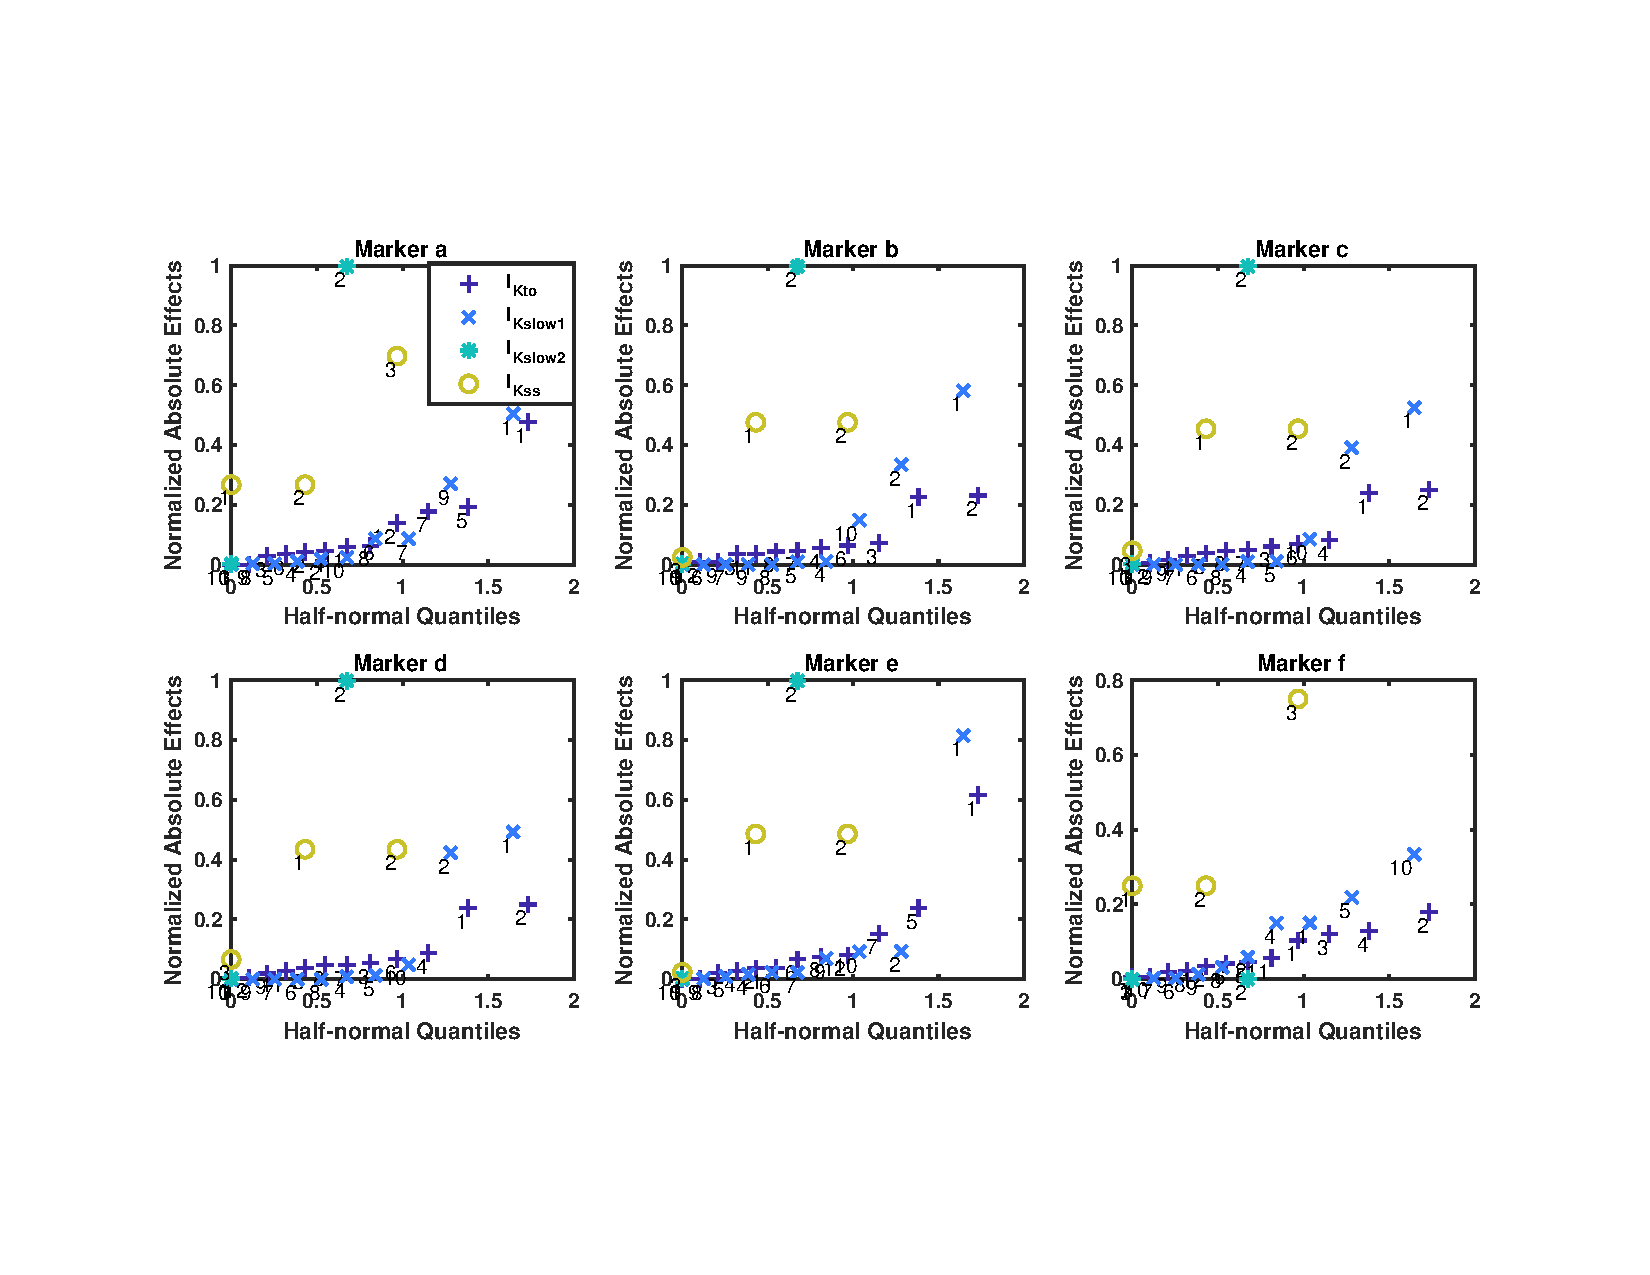
\includegraphics{figs/half-norm.pdf}
    \caption{Half-normal plots of factorial effects of parameters on the six maker points.}
    \label{fig:half-norm}
\end{figure}

\textbf{Figure~\ref{fig:calib_param}} shows the selected parameters, highlighted in different colors according to their functional roles in channel kinetics. We categorized the calibration parameters into four classes: The red represents the voltage-threshold parameters and the green voltage slopes, controlling the voltage dependence, the blue scale factors of kinetic functions, and purple time-constant shifters. Note that the voltage-dependence parameters in red and green appear multiple times across different equations. This parsimonious model design is intended to maximize the structural regularization to minimize overfitting.
\begin{figure}[!ht]
    \centering
    \includegraphics{figs/calib_param.pdf}
    \caption{Selected parameters from the sensitivity analysis, highlighted in different colors according to their functional roles in channel kinetics.}
    \label{fig:calib_param}
\end{figure}

\subsection{Model Fitness}
We compared three nonlinear optimization algorithms satisfying box constraints: BFGS, sequential quadratic programming (SQP), and active set methods. \textbf{Fig~\ref{fig:model_fitness}A} and \textbf{C} shows values of the objective function (sum of RMSEs) of the three optimization algorithms for WT and MGAT1KO, respectively. The three algorithms barely showed differences in the objective values. We compared the actual model predictions and experimental potassium I\textsubscript{K} traces in \textbf{Figure~\ref{fig:model_fitness}B} and \textbf{D} to validate the model calibration results further. Representative data were selected randomly for each group and plotted at -30 mV and 50 mV voltage steps to illustrate discrepancies at low and high voltages. Sum of RMSEs values are lower in MGAT1KO than WT in general, because magnitudes are smaller for the disease group. Calibration results of the BFGS algorithm will be used in analysis of kinetics modeling in the rest the sections. 
\begin{figure}[!ht]
    \centering
    \includegraphics{figs/model_fitness_4half4.pdf}
    \caption{Bar graphs of the sum of RMSEs of (A) WT and (C) MGAT1KO, and representative actual fitness between model outputs and experimental I\textsubscript{K} recordings (in red) at -30 mV and 50 mV voltage steps of (B) observation 26 in WT and (D) 4 in MGAT1KO.}
    \label{fig:model_fitness}
\end{figure}

\subsection{Kinetics Modeling} \label{s:results.kinetics}
The \textit{in-silico} modeling predicts that reduced N-glycosylations cause significant changes in channel kinetics and gating behavior. \textbf{Figure~\ref{fig:kinetics_ikto}} presents the \textit{in-silico} modeling results of showing kinetics variables to voltage relationships of K\textsubscript{v}4.2. There is a slight rightward shift in steady-state activation (SSA) values along the voltage axis (\textbf{Figure~\ref{fig:kinetics_ikto}A}), and steady-state inactivation (SSI) is reduced up to 0.2 at voltages lower 0 mV (\textbf{Figure~\ref{fig:kinetics_ikto}B}). Activation and inactivation time constants $\tau_{a}^{(1)}$ and $\tau_{i}^{(1)}$ to voltage relationships are shown in \textbf{Figure~\ref{fig:kinetics_ikto}C} and \textbf{D}. $\tau_{a}^{(1)}$ for MGAT1KO is higher in range of $>$ -10 mV than WT. $\tau_{i}^{(1)}$ for MGAT1KO is slightly shifted toward left. The shifts in SSA and SSI likely cause the reductions in I\textsubscript{Kto} magnitudes, and the increases time constants explain delays in the decaying phase observed in the \textit{in-vitro} experiments.
\begin{figure}[!ht]
    \centering
    \includegraphics{figs/kinetics_ikto.pdf}
    \caption{Kinetics functions in I\textsubscript{Kto} and their relationships to voltage. (A) steady-state activation, (B) steady-state inactivation, (C) time-constant activation, and (D) time-constant inactivation.}
    \label{fig:kinetics_ikto}
\end{figure}

\textbf{Figure~\ref{fig:kinetics_rec}} shows kinetics modeling results of the channels producing the delayed rectifier currents, I\textsubscript{Kslow1} and I\textsubscript{Kslow2}, and steady-state current I\textsubscript{Kss}. The most prominent result is that the time constants of I\textsubscript{Kslow1} are estimated to be significantly slow in MGAT1KO $\sim$ 3.4 and 235.8 ms (\textbf{Figure~\ref{fig:kinetics_rec}D} and \textbf{E}). Similar to I\textsubscript{Kto}, there is a small rightward shift in SSA at voltaged $>$ -10 mV for MGAT1KO. SSI is also shifted $\sim$ 10 mV to the right. Slow time constants and increased SSI are likely to address the flattened shape of MGAT1KO currents as illustrated in \textbf{Figure~\ref{fig:model_fitness}D}). Time constant inactivation of I\textsubscript{Kslow2} (\textbf{Figure~\ref{fig:kinetics_rec}C}) and activation of I\textsubscript{Kss} (\textbf{Figure~\ref{fig:kinetics_rec}F}) do not show significant differences between the two groups.
\begin{figure}[!ht]
    \centering
    \includegraphics{figs/kinetics_rec.pdf}
    \caption{Kinetics functions and their relationships to voltage of I\textsubscript{Kslow1} (A) steady-state activation, (B) steady-state inactivation, (D) time-constant activation, (E) time-constant inactivation, (C) I\textsubscript{Kslow2} time-constant inactivation, and (F) I\textsubscript{Kss} time-constant activation.}
    \label{fig:kinetics_rec}
\end{figure}

\subsection{Parameter Distributions Between WT and MGAT1KO} \label{s:results.distribution}
We estimated distributions of the calibrated kinetic parameters to analyze the impacts of reduced N-glycosylation further. \textbf{Figure~\ref{fig:hist_pkto}} shows the distributional differences of the kinetic parameters in the K\textsubscript{4.2} model between the two group. A notable fact about the figure is that MGAT1KO shows small variances for Parameters 1, 5, and 7 in transition $\alpha_{a}$ and $\beta_{a}$, which control kinetics activation of I\textsubscript{Kto}. Reduced glycosylation affects activation gating that plays a vital role in I\textsubscript{Kto}, as it is characterized by a high peak at the early depolarization and rapid inactivation. In addition, MGAT1KO causes a leftward shift in the distribution of the maximum conductance $G_{\mathrm{Kto}}$, resulting in smaller conduction than WT in general. It is likely due to the observed current reductions in MGAT1KO.
\begin{figure}[!ht]
    \centering
    \includegraphics{figs/hist_pkto.pdf}
    \caption{Distribution estimations of calibration parameters in the K\textsubscript{Kto} model.}
    \label{fig:hist_pkto}
\end{figure}

\textbf{Figure~\ref{fig:hist_prectifiers}} shows distribution estimations of the calibration parameters in the rectifier and steady-state currents models. \textbf{Figure~\ref{fig:hist_prectifiers}A} shows significant distributional differences in Parameters 9 and 10, which control time constants of I\textsubscript{Kslow1}. It is compatible with the previous observations of significant differences in time constants to voltage relationships of I\textsubscript{Kslow1} between WT and MGAT1KO. There are slight shifts in Parameters 1 and 4 of I\textsubscript{Kslow1} that affect steady-state activation. The voltage-threshold parameter for MGAT1KO in steady-state inactivation has higher densities at low values around 30 than WT, which has the peak mode around 48. It accounts for the shift at low voltages less than 0 mV in SSI. The maximum conductance $G_{\mathrm{Kslow1}}$ of MGAT1KO is centered around relatively small values compared to WT. This leftward shift in the maximum conductance is also observed in I\textsubscript{Kslow2} (\textbf{Figure~\ref{fig:kinetics_rec}B}). Although there is a difference in variance of $G_{\mathrm{Kss}}$, the two groups have similar means around 0.03 (i.e. WT: $0.0375\pm0.0027$ vs MGAT1KO: $0.0325\pm0.015$). It is compatible with the observation that I\textsubscript{Kss} does not show significant reductions. 
\begin{figure}[!ht]
    \centering
    \includegraphics{figs/hist_prectifiers.pdf}
    \caption{Distribution estimations of calibration parameters in (A) the I\textsubscript{Kslow1} model, (B) the I\textsubscript{Kslow2} model, and (C) the I\textsubscript{Kss} model.}
    \label{fig:hist_prectifiers}
\end{figure}

\subsection{Low-dimensional Embedding and Visualization}
We aggregated calibration results into one to analyze the parameters in a collective way. It resulted in a $61\times20$ matrix (i.e., 31 observations in WT and 30 in MGAT1KO, and there are 20 calibration parameters). Then we applied t-distributed stochastic neighbor (t-SNE) embedding to encapsulate the high-dimensional data into three-dimensional space so that we could visualize each data point. \textbf{Figure~\ref{fig:cluster}} presents the visualization of the t-SNE embedding of the calibration results. It shows not only clear differences between the two groups but also variances of cells (i.e., data points) within the groups and across the entire dataset.
\begin{figure}[!ht]
    \centering
    \includegraphics{figs/cluster.pdf}
    \caption{t-SNE embedding of calibration parameters.}
    \label{fig:cluster}
\end{figure}

\section{Conclusions}\label{s:conclusions}
We propose a novel data assimilation framework of voltage-gated K\textsuperscript{+} channels that combines experimental data with computer models guided by simulated channel kinetics to investigate disease-altered cardiac electrical signaling. This approach provides a complementary tool to physical experiments that are limited in their ability to determine molecular-level channel kinetics rigorously and provide predictive insights. Traditional methods, based on curve-fitting, do not consider interactions of various gating variables across isoforms and dynamics of kinetics according to changes in protocols. The proposed method focuses on more comprehensive modeling of underlying channel kinetics of K\textsubscript{v} isoforms than traditional approaches. Experimental results show the strong potential of the proposed framework to discover channel kinetics from various angles. Predictions of kinetics variables to voltage relationships provide information about changes in the voltage dependence of channels. In addition, calibrated parameters of the computer models present a micro-level analysis of channel gating. The embedding method allows visualizing the variability of each cell. In summary, the proposed framework paves a new way for investigating the electrical signaling of potassium channels and heart diseases. 

\if0\blind{
\section*{Acknowledgements}
The authors acknowledge the generous support from the funding agency of XYZ and funding list} \fi

\bibliographystyle{chicago}
\spacingset{1}
\bibliography{IISE-Trans}
	
\end{document}
